% Created 2024-04-28 Sun 16:43
% Intended LaTeX compiler: pdflatex
\documentclass[letterpaper, 10pt, twocolumn]{article}
                      \usepackage{lmodern} % Ensures we have the right font
\usepackage[T1]{fontenc}
\usepackage[utf8]{inputenc}
\usepackage{graphicx}
\usepackage{amsmath, amsthm, amssymb}
\usepackage[table, xcdraw]{xcolor}
\renewcommand{\thesection}{\Roman{section}}
\renewcommand{\thesubsection}{}
\renewcommand{\thesubsubsection}{}
\definecolor{bblue}{HTML}{0645AD}
\usepackage[colorlinks]{hyperref}
\hypersetup{colorlinks, linkcolor=blue, urlcolor=bblue}
\usepackage{titling}
\setlength{\droptitle}{-6em}
\setlength{\parindent}{12pt}
\setlength{\parskip}{0em}
\usepackage[stretch=10]{microtype}
\usepackage{hyphenat}
\usepackage{ragged2e}
\usepackage{subfig} % Subfigures (not needed in Org I think)
\usepackage{hyperref} % Links
\usepackage{listings} % Code highlighting
\usepackage[top=1in, bottom=1.00in, left=0.85in, right=0.85in]{geometry}
\renewcommand{\baselinestretch}{1.00}
\usepackage[explicit]{titlesec}
\pretitle{\begin{center}\fontsize{20pt}{20pt}\selectfont}
\posttitle{\par\end{center}}
\preauthor{\begin{center}\vspace{-6bp}\fontsize{12pt}{12pt}\selectfont}
\postauthor{\par\end{center}\vspace{-25bp}}
\predate{\begin{center}\fontsize{12pt}{12pt}\selectfont\vspace{1em}}
\postdate{\par\end{center}\vspace{0em}}
\titlespacing\section{0pt}{5pt}{5pt} % left margin, space before section header, space after section header
\titlespacing\subsection{0pt}{5pt}{2pt} % left margin, space before subsection header, space after subsection header
\titlespacing\subsubsection{0pt}{5pt}{-2pt} % left margin, space before subsection header, space after subsection header
\usepackage{enumitem}
\setlist{itemsep=-2pt} % or \setlist{noitemsep} to leave space around whole list
\usepackage{listings}
\author{jmowry4@vols.utk.edu}
\date{4/16/24}
\title{\textbf{Maximizing Requests per Second on a Single Thread through \texttt{io\_uring}}\\\medskip
\large Jackson Mowry}
\hypersetup{
 pdfauthor={jmowry4@vols.utk.edu},
 pdftitle={\textbf{Maximizing Requests per Second on a Single Thread through \texttt{io\_uring}}},
 pdfkeywords={},
 pdfsubject={},
 pdfcreator={Emacs 29.3 (Org mode 9.7)}, 
 pdflang={English}}
\begin{document}

\maketitle
\section{Abstract}
\label{sec:org178dc8a}
\textbf{This research paper investigates the transformative potential of \texttt{io\_uring} in scaling HTTP web servers to accommodate the needs of numerous concurrent clients. Despite the extensive exploration of various scaling techniques, little attention has been paid to the potential paradigm shift that \texttt{io\_uring} may introduce in asynchronous I/O architectures. \texttt{io\_uring} enables the handling of workloads traditionally confined to highly parallelized systems. This paper aims to explore the implications of \texttt{io\_uring} on asynchronous I/O systems, shedding light on its promise for enhancing server scalability and performance in the face of ever increasing demands.}
\section{Introduction}
\label{sec:orgbbe265d}
Web servers are a class of software that sit between nearly every interaction a client makes on their device, and access to the files hosted on a server. Despite this fact their implementations mainly use software designs of the past, due to the fact that for most use cases they are ``good enough''. It is true that even a naive HTTP server can serve thousands of requests per second, which easily surpasses the needs of most users, but when it comes time to scale up the same architecture only has two ways to scale. The server can either be rewritten to take advantage of multiple CPU cores, or it can have multiple instances running behind a load balancer.

The root of this issue lies in the fact that these workloads are still inhrently synchronous at some level (excluding \texttt{aio}), which leads to large requests stalling the server. \texttt{io\_uring} brings a true asynchronous io system to the table with its introduction into the Linux kernel (version 5.1). An exciting new space for high performance single core servers now exists, in this paper we will see how \texttt{io\_uring} can fill that gap. To date \texttt{io\_uring} has not been implemented in mainstream web server applications, this paper serves to illuminate the potential benefits, to both speed and latency, of the latest in asynchronous io technology.
\section{Previous Work}
\label{sec:orgbe0803d}
\subsection{{\bfseries\sffamily TODO} }
\label{sec:org18bd5ae}
\section{Asynchronous IO}
\label{sec:org6e70200}
Most if not all system calls used in day to day software are considered ``blocking'', meaning they will only return once the entire function has finished executing. This model allows for programs to not having to worry about order of execution, as they know their program will run top to bottom without skipping a step. However, large web servers simply cannot afford to spend the time waiting for each system call to execute to completion. To avoid this problem of blocking programmers may choose to design their software around asynchronous IO.

For most applications it may not make sense to perform all system calls asyncronously. We certainly want slower system calls to complete in the background, but the added overhead of an asynchronous system call may make faster calls worse. We expect to see greater differences in throughput for large files as they would stall the server while attempting to read/write data that may not fit in a single block/page.
\section{\texttt{aio}}
\label{sec:org3133455}
The \texttt{aio} system in Linux has two implementations, POSIX compliant, and the Linux implementation. Both systems suffer the same issue, they are intended to work with regular files, and as such don't play well with sockets. glibc creates a thread pool to perform regular synchronous io off the main thread, giving the illusion of asynchronosity to the user-space program.

\texttt{aio} is also very limited in scope, only offering real support for read and write calls. This means that without splicing together features from different asynchronous IO frameworks an application will still have to rely heavily on blocking system calls.

For all of these reasons \texttt{aio} is generally avoided in application code.
\section{\texttt{epoll}}
\label{sec:orgfdff83b}
\texttt{epoll} is kernel based implementation of \texttt{poll}, with both providing a way to monitor a range of file descriptors, and alerting the user when one or many are ready for IO. It has become a common architecture for web servers and other asychronous io systems to be built on top of. Most notably to implement the primatives golang's \texttt{net/http} package is built upon, and \texttt{libuv} which powers the Node.js event loop.

\texttt{epoll} expands on the original ideas of poll by sharing a list of file descriptors between the user and kernel, preventing the need for data to be copied back and forth. When any number of file descriptors are ready for IO they will be placed in a separate shared list, which the user can then perform the desired action on.

This architecture allows for a single thread to handle large numbers of active file descriptors, only slowing down to perform the synchronous operations like reading or writing. The actual implementation does not allow for asynchronous sending or recieving of data, merely alerting the user when those operations can be performed without blocking. One downside of \texttt{epoll} is that it does not behave consistently across file descriptors of different types. While it is true that recieving data from a socket can block, which \texttt{epoll} is aware of, regular files do not exhibit the same behavior.

Due to \texttt{epoll}'s handling of regular files they will always be placed on the ready list immedietly. On Linux read and write calls to a file should not block, but as we all know this is not true. You can make a write call and expect it to complete instantly, but if the kernels write cache is full, you will have to wait. The same goes for a read call which can blocked if the file is on a slow drive.
\section{\texttt{io\_uring}}
\label{sec:org308d25d}
\texttt{io\_uring} is the latest attempt at adding asynchronous operations to Linux. Its design makes it obvious that it the designer learned from many of the shortcomings of \texttt{aio}. Not only does \texttt{io\_uring} provide a common interface across all types of file descriptors, it also implements most systems calls in an asyncronous fashion.

The design can be broken down into two distinct parts, a job submission queue, and a job completion queue, both implemented via ring buffers shared between the kernel and user space. At a basic level each submission is a combination of an op code defining which system call to perform, and the associated arguments. If the user desires to keep track of a job they can associate user data with a submission, which takes the form of an 64-bit integer, commonly used to hold a pointer. The implementation garuntees that user data will not be modified.

Once a job is complete it is placed in the completion queue, which an application can pull from. Completions have 2 main fields to pay attention to: a result code, and the associated user data. The result code is analogous to the return value from regular blocking system calls with one exception. Due to the concurrent execution of submissions the system cannot garuntee that the \texttt{ERRNO} associated with each system call will still be properly set when a user recieves a completion. Instead, \texttt{ERRNO} is placed in the completion struct, with its value negated so that it will not be confused with a successful execution.

\texttt{io\_uring} also offers one distinct advantage over the other asynchronous io methods presented here. Jobs can be submitted through a system call, or by having the kernel continuously poll the submission queue using a separate thread. This allows for a program to operate entirely in user space, avoiding system calls which have become even more costly in the age of speculative execution mitigations. In systems where response time is the highest concern, submission queue polling will likely be the best choice due to eliminating a system call per request. We will explore both methods of job submission to see where their advantages lie.

Being the latest in the asyncronous IO space \texttt{io\_uring} is still lacking some features. Most notably is missing system calls, and event notification on a submission/completion level. Most missing system calls can be implemented without changing the underlying system, with the remaining few not being necessary to implement asynchronously.
\section{System Calls}
\label{sec:org06be674}
One of the major mitigations put into place after the speculative execution attacks were discovered (spectre and meltdown) was isolation of kernel and user space memory. This slows system calls as they must switch into a different address space to perform the operation, and switch back once they're done.

To mitigate this, modern software systems have transitioned to a model where system calls are avoided, sometimes entirely. The most obvious implementations of this are systems that manage memory allocations themselves, or those that manage files using shared memory.

\texttt{io\_uring} allows the program to avoid system calls upon submission, meaning that a system can work entirely in userspace, without the need for costly system calls. This reduces the number of system calls from at a minimum 4 (accept, read, write, close) in a synchronous server, to a potential 0 in an \texttt{io\_uring} based approach. For a simple file server the only system call that is still required is \texttt{pipe}, which does not have an asynchronous implementation yet.

Allowing system calls to proceed asynchronously also allows for a program to handle clients with heavy requests without blocking clients with lighter weight requests. This is a major advantage over synchronous servers where either an entire program is blocking reading/writing a file, or a thread is held up waiting. This can slow the overall throughput of these systems, whereas an asynchronous implementation would proceed handling other clients while a file is being read.

Many modern web servers also try to combat the cost of system calls by using auxiliary threads to handle either entire requests, or smaller portions. This approach works until a certain point, as the overthread of spawning an operating system thread is non-trivial. The best approach will likely vary application to application, as certain applications may require heavy synchronous computations, which a single thread would not be able to handle.
\section{Methods \& Implementation}
\label{sec:org547e821}
Testing will include an \texttt{epoll} server, four distinct \texttt{io\_uring} servers, and a sixth synchronous server using \texttt{poll}. Servers will parse a request, open a file, respond with the appropriate headers, send the file, and finally close the connection. Performance testing using \texttt{wrk} at \{1, 4, 8, 16, 32, 64, 128, 256, 512, 1024, 2048, 4096, 8192\} concurrent connections run over 30 seconds, with the mean of 3 runs reported for each metric.

For testing four \texttt{io\_uring} based servers will be compared. For a more realistic general purpose web server (uring simple) example, only the accept, read, and close system calls will be replaced with their asynchronous counterparts, with the rest of the work handled synchronously. The application follows a simple state machine where a connection is either in \texttt{ACCEPT}, \texttt{READ}, or \texttt{WRITE/CLOSE}.

The complete \texttt{io\_uring} server will replace every system call (except for \texttt{pipe} which does not yet exist) with their asynchronous versions (uring full). The state machine follows a similar pattern adding \texttt{CLOSE\_FILE}, \texttt{CLOSE\_SOCKET}, \texttt{CLOSE\_PIPE}, \texttt{OPEN}, \texttt{SPLICE}, \texttt{STATX}, and \texttt{SEND}. Each of these servers will also have submission queue polling enabled (uring simple + SQP) (uring full + SQP) as an additional observation point. 
\section{Results}
\label{sec:org0ffcd02}
\subsection{Latency}
\label{sec:orgc05c14d}
\begin{figure*}
\centering
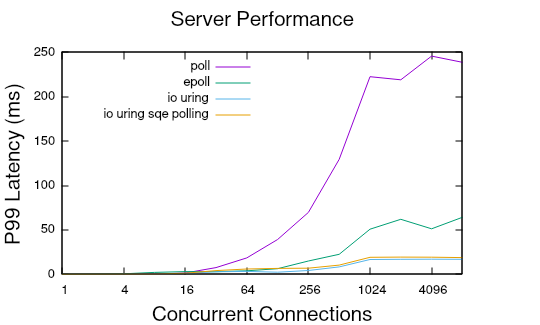
\includegraphics[width=4.5in]{./p99_latency.png}
\end{figure*}

As expected, the synchronous \texttt{poll} based server experiences substantial growth in latency as the number of concurrent request in increased. This is due to the fact the scanning the list of watched file descriptors happens in linear time as each is checked for a \texttt{POLLIN} event. The \texttt{epoll} server is able to maintain a similar latency to either \texttt{io\_uring} server until 128 concurrent request when it begins to climb rapidly. Latency continues to grow with connections, and would be expected to continue rising.

Both \texttt{io\_uring} servers exhibit similar P99 latency, quickly reaching a plateau around 25ms from 1024 concurrent requests and beyond. One of the key benefits of \texttt{io\_uring} is its ability to handle massively concurrent workloads, as observed with either implementation. Submission queue polling increases latency by a fixed amount across the entire test range, the change seems to have the largest impact when serving small files, as was predicted. For the simple and full \texttt{io\_uring} server enabling polling dropped latency by 67\% and 53\% respectivly.

\begin{center}
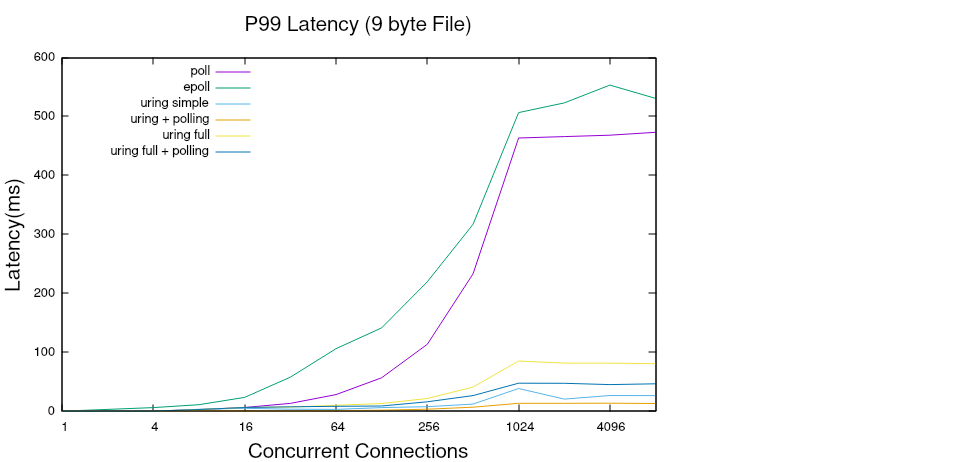
\includegraphics[width=5in]{tiny_p99.png}
\end{center}

\begin{center}
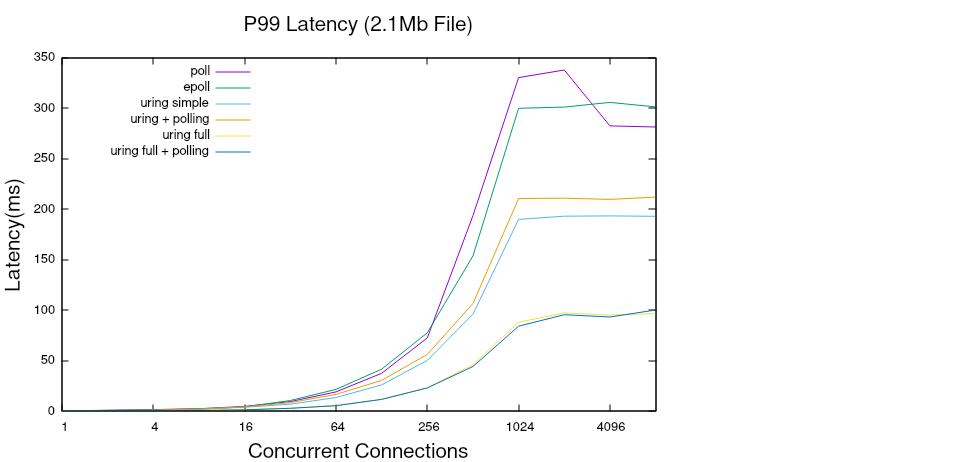
\includegraphics[width=5in]{large_p99.png}
\end{center}

While serving small files still benefits substantially from \texttt{io\_uring}, the simple \texttt{io\_uring} server beats a full server by a factor of 2x. A small file tends to be less performance bound by disk IO, as the entire file can easily be read and written in a single page. Moving up to a medium sized file (12Kb) we see that the gap between either \texttt{io\_uring} remains about the same, just around 2x. It is not until the large file is requested that a full \texttt{io\_uring} server begins to show its advantages. At a full 8192 connection load the simple \texttt{io\_uring} server peaks at 200ms of latency, whereas the full \texttt{io\_uring} server just begins to push 100ms. Either synchronous server continues to climb in latency up until a peak of 300ms at full load.
\subsection{Throughput}
\label{sec:org1c910b8}

\begin{center}
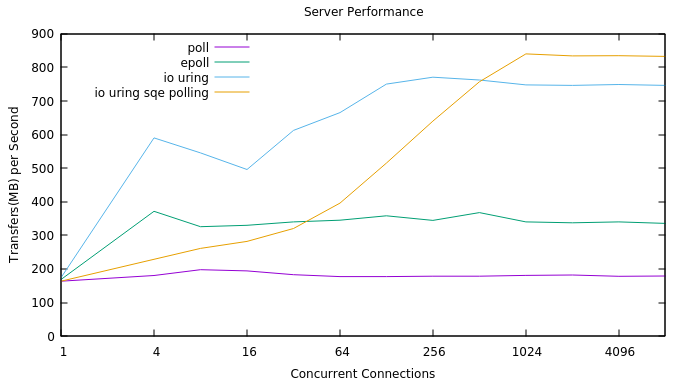
\includegraphics[width=.9\linewidth]{mbps.pn.png}
\end{center}
\begin{center}
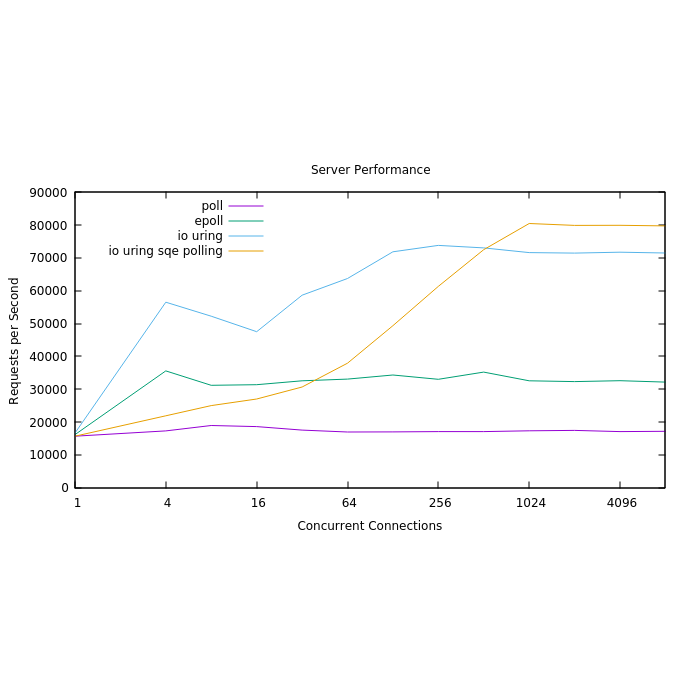
\includegraphics[width=.9\linewidth]{rps.png}
\end{center}

Throughput of the synchronous server follows our expectations, a nearly flat line across the entire testing range. The rate at which we can push data over the wire is entirely limited by the fact that each request is handled one at a time, which is entirely dependent on the time on which we are blocked in system calls. For simple applications this approach may be enough to handle the workload, and it comes with the upside that a \texttt{poll} implementation is a much simpler architecture.

\texttt{epoll} exhibits nearly the same behavior as the poll based implementation, only at a higher overall throughput. We see no degradation in throughput for either server up to 8192 concurrent request. The advantage for \texttt{epoll} comes in the fact that it's ``work queue'' is only populated with requests that have data ready, meaning that each file descriptor can have work done without having to check its status.

A basic \texttt{io\_uring} server without submission queue polling quickly reaches its maximum throughput at 128 concurrent requests, which the server is able to maintain all the way up through 8192 concurrent requests. This equates to a maximum throughput of around 750MB/s, or \textasciitilde{}6Gbit/s, serving a 12KB text file to each client. When submission queue polling is enabled we see an interesting shift in throughput. A much lower throughput is seen at lower concurrent requests, which quickly jumps past the original implementation at 512 concurrent requests. From 512 requests and beyond a gap of just under 10,000 requests per second is maintained. This equates to a gap of around 100MB/s, or 0.8Gbit/s.

As suspected the fully asynchronous server is still slower for medium sized files. The performance scales in the same manner at half the overall throughput. We observe similar performance impacts from enabling submission queue polling, only overcoming non-polling past 512 concurrent requests as seen in the previous example.

\begin{figure*}
\centering
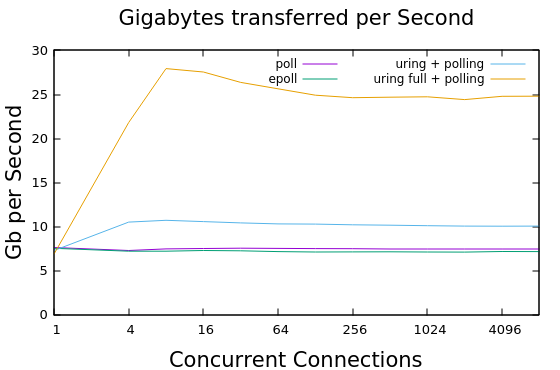
\includegraphics[width=4.5in]{gbps.png}
\end{figure*}

Testing with large file sizes begins to highlight the advantages from the newer \texttt{io\_uring} system. When clients request a 2.1Mb file we finally begin to see that the full \texttt{io\_uring} server has major advantages. Without blocking each request on a single synchronous path we greatly increase throughput, and decrease latency. Both synchronous servers, and the simple \texttt{io\_uring} server spend the majority of their runtime blocked in system calls, meaning that even though we have thousands of connected clients, we cannot concurrently send any information to multiple clients.

The general flow of a request is to first open \texttt{stat} the file to gather information, open the file for reading and then using either \texttt{sendfile}, or a combination of pipes and splicing to achieve the same effect. When using a single thread in a synchronous context we see a large increase in latency due to this linear pipeline of information transfer. We must wait until the entire file (and corresponding headers) have been passed off to the kernel to send. This results in our latency being enitrely determined by the speed at which a single client can be served.

In a fully asynchronous context, many thousands of clients can connect at the same time, with each of their requests being processed concurrently. The largest contributing factor to decreased throughput (and thus increased latency) is the sending of the large 2.1Mb file, which is entirely mitigated when using asynchronous IO. This results in our fully asynchronous server beating \texttt{epoll} by 3.5x, and a simple \texttt{io\_uring} server by 2.5x. At 8 concurrent clients the fully asynchronous implementation achieves an average throughput of 27.94GB/s, settling in to just around 24.8GB/s for the remaining tests.

We see the opposite results when testing a smaller 9 byte file, as the overhead of processing system calls asynchronously greatly decreases overall throughput. The best performer with small files was the simple \texttt{io\_uring} implementation with submission queue polling enabled, which managed 8.79MB/s at 8192 concurrent connections. Our fully asynchronous server was able to achieve just under half the throughput (3.84MB/s), still beating either synchronous server (\textasciitilde{}1.30MB/s).
\section{Discussion}
\label{sec:org7cd65e3}
Either asynchronous implementation offers obvious advantages over an entirely synchronous server. \texttt{epoll} offers an interesting middle ground where the architecture is simpler, at the cost of reduced throughput. However, \texttt{epoll} has better portability when if the application needs to run on the family UNIX based systems. Linux has \texttt{epoll}, while MacOS and BSD both have \texttt{kqueue}, which offers a similar API for performing asynchronous operations on file descriptors. \texttt{epoll} has also been around since Linux kernel version 2.5 (2002), meaning resources and documentation are more widely available.

As discussed before, one potential disadvantage with \texttt{epoll} is that it only works well with sockets, or files opened in an unbuffered/direct mode. If an application needs to do more than accept an incoming connection on a socket and send back a response, \texttt{epoll} will not be useful for other operations. \texttt{io\_uring} on the other hand offers a uniform interface for the entire range of IO operations. This consistent handling of different file descriptors allows for the programmer to simplify their application to a more robust state machine.

A fully asynchronous server is able to scale in both throughput and latency, which is desireable for many applications. This increase in performance also comes with the simplicity of running on a single user space thread. A single threaded application generally limits the need for concurrency control mechanisms, which can slow the execution of a program.

\texttt{io\_uring} has shown that with its superior implementation it can out perform the contemporary way we build web servers. Showing a 75.95\% improvement (85.01\% for SQ polling) in throughput over the \texttt{epoll} based server at 8192 concurrent requests when serving a 12Kb file. The worst case latency of an \texttt{io\_uring} server also scales better than \texttt{epoll}, exhibiting 1/4 the latency at 8192 concurrent requests.

The general performance gap only grows as the response size does as well. When serving a 9 byte file \texttt{io\_uring} exhibits a 2x increase in throughput, which grows to over 2.5x at 12Kb, and finally 3.5x for a 2.1Mb file. This follows the long known trend that asynchronous operations help IO bound applications scale. As file size increases we would expect to see the same trend of decreased latency and increase throughput.
\section{Future Work}
\label{sec:org96ebccc}
More work is needed to explore the different performance impacts of various asynchronous calls through \texttt{io\_uring}. Theoretically, a server performing very few systems calls should outperform one doing many system calls, but as we have observed, this is not always the case. Once a few more of the key systems calls have been implemented (pipe, and sendfile specifically) performance testing should once again be performed.
\section{Cite}
\label{sec:org8c63c17}
\url{https://www.kernel.org/doc/ols/2003/ols2003-pages-351-366.pdf}
\url{https://www.landley.net/kdocs/mirror/ols2004v1.pdf\#page=215}
\url{https://darkcoding.net/software/linux-what-can-you-epoll/}
\url{https://darkcoding.net/software/epoll-the-api-that-powers-the-modern-internet/}
\end{document}
